\documentclass[UTF8]{ctexart}
\usepackage{fullpage}
\usepackage{times}
\usepackage[normalem]{ulem}
\usepackage{multirow}
\usepackage{fancyhdr,graphicx,amsmath,amssymb, mathtools, scrextend, titlesec, enumitem}\usepackage[pdftex]{hyperref}
\usepackage[ruled,vlined]{algorithm2e}
\usepackage{parskip}
\usepackage{listings}
\usepackage{amsmath}
\usepackage{physics}
\usepackage{bbm}
\usepackage{titling}
\usepackage{bm}
\usepackage{geometry}
\geometry{top=1cm, left=1cm, bottom=1.5cm, right=1.5cm, margin=1cm}
\newcommand{\varvec}[2][n]{#2_1,\ldots, #2_#1}
\newcommand{\Var}{\mathrm{Var}}
\newcommand{\Bias}{\mathrm{Bias}}
\newcommand{\Cov}{\mathrm{Cov}}
\newcommand{\E}{{\rm I\kern-.3em E}}
\newcommand{\Binomial}{\mathrm{Binomial}}
\newcommand{\Bernoulli}{\mathrm{Bernoulli}}
\newcommand{\Poisson}{\mathrm{Poisson}}
\newcommand{\Normal}{\mathcal{N}}
\newcommand{\one}{\mathbbm{1}}
\newcommand{\Beta}{\text{Beta}}
\newcommand{\BetaPDF}{\text{Beta}}
\newcommand{\GammaPDF}{\text{Gamma}}
\newcommand{\Uniform}{\mathrm{Uniform}}
\newcommand{\QED}{\newline \mbox{} \hfill $\blacksquare$}
\newcommand{\Real}{\mathbb{R}}
\newcommand{\Sgn}{\mbox{Sgn}}
\renewcommand*{\arraystretch}{1.4}
\newtheorem{theorem}{Result}
\newtheorem{definition}{Definition}
\lstset{frame=tb,
	language=Python,
	aboveskip=3mm,
	belowskip=3mm,
	showstringspaces=false,
	columns=flexible,
	basicstyle={\small\ttfamily},
	numbers=none,
	stringstyle=\color{mauve},
	breaklines=true,
	breakatwhitespace=true,
	tabsize=3
}

\graphicspath{ {./img} }



\title{乐理(Music Theory)}

\begin{document}
	\maketitle
	

五线谱(Staff)开始有谱表(Clef)是音高的锚点,比如
高音谱表(Treble clef)又名G谱表(G Clef)表示从下面数第二条线是G。
而低音谱表(Bass clef)又名F Clef,表示从上面数第二条线是F
\begin{center}
	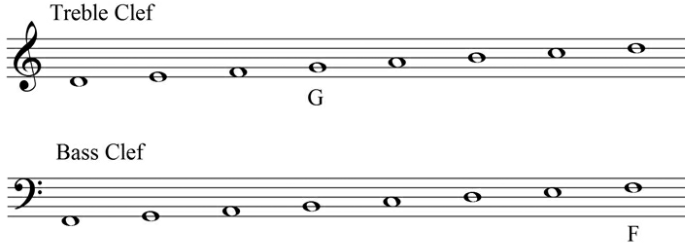
\includegraphics[scale=0.5]{clef.png}
\end{center}


音高(pitch)是单一频率的声音,比如
A1 (55Hz), A2(110Hz), A3(220Hz), A4(440Hz), A5(880Hz), A6(1760Hz), A7(3520Hz)
\begin{center}
	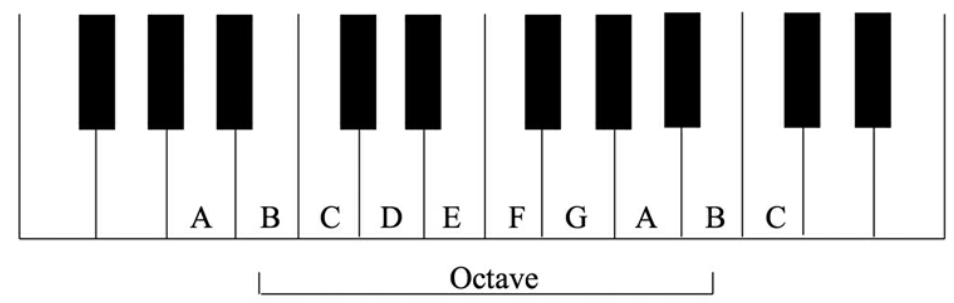
\includegraphics[scale=0.5]{piano_octave.png}
\end{center}
一个八度(Octave)由12个半音(half step)组成。半音是相邻的钢琴键(B到C,A到A\#)。全音(Whole Step)是隔了一个键(比如A到B)。

半音音阶(Chromatic Scale)是一个八度内包含全部12个半音(白键+黑键)

升号(Sharp)和降号(Flat)都是临时记号(Accidentals)

音符长短(Duration)
\begin{center}
	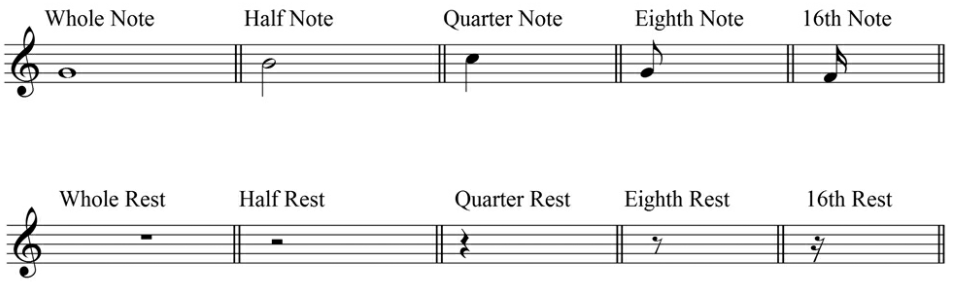
\includegraphics[scale=0.5]{duration.png}
\end{center}

拍型(Meter): 一下小节(Measure/Bar)里不同节拍(Beat)有不同强弱规律
\begin{center}
	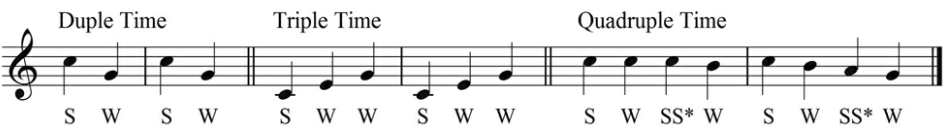
\includegraphics[scale=0.5]{meter.png}
\end{center}

时间记号(Time Signature)比如(6/8)表示每个小节有相当于6个8分音符的音符,4/4则表示4个4分音符。
下图C表示Common即为4/4, C斜杠表示2/2。
\begin{center}
	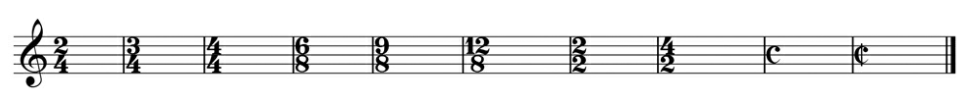
\includegraphics[scale=0.5]{time_signature.png}
\end{center}
 注意6/8,9/8, 12/8是复拍子(Compound Time)。在6/8里一拍是四分音符加点,而不是8分音符(看下方例子)。如果第一个数字是3的倍数(6,9,12等)就是复拍子
\begin{center}
	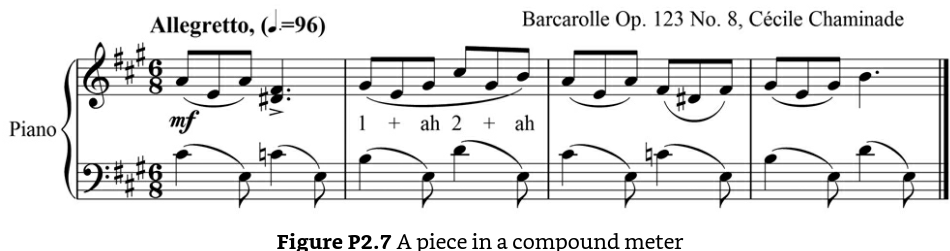
\includegraphics[scale=0.5]{compound_time.png}
\end{center}

强拍(Downbeat)是小节第一拍, 弱拍(Upbeat)是最后一拍
\begin{center}
	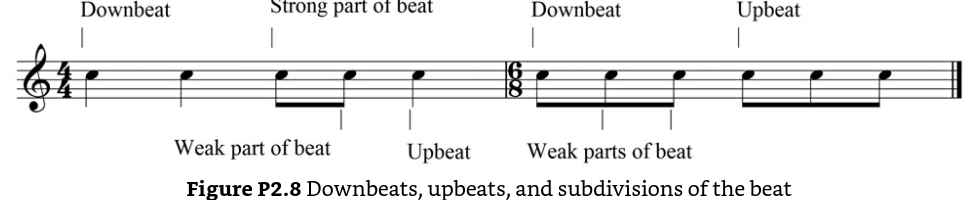
\includegraphics[scale=0.5]{downbeat_upbeat.png}
\end{center}

将音符连在一起的横线或斜线被称为“符梁”或“符杠”(Beam)。 将八分音符和十六分音符用符梁组合在一起(Beaming)取决于时间记号,比如6/8,每个小节是两拍,所以8分音符会每三个连成一组(如图2.7)

\end{document}